\documentclass{article}
\usepackage[top=2.5cm, left=3cm, right=3cm, bottom=2.5cm]{geometry}
\usepackage[utf8]{inputenc}
\usepackage{alphabeta}
\usepackage{fullpage}
\usepackage{amsmath,amssymb}
\usepackage{tikz}
\usepackage{listings}
\usepackage{graphicx}
\usepackage{float}
\usepackage{subcaption}
\usepackage{booktabs}
\usepackage[colorlinks=true,linkcolor=black,citecolor=black,urlcolor=black]{hyperref}

\linespread{1.15}
\title{Pet Image Classification - CV 2025}
\author{Marios Giannopoulos\\Student ID: 1115202000032}
\date{2026-02-02}

\begin{document}
\maketitle
\tableofcontents

\section{Introduction}
\label{sec:introduction}
\phantomsection

This assignment implements two alternative computer vision pipelines for classifying pet breed images (6 classes: Abyssinian, Bengal, Birman, Boxer, English Cocker Spaniel, German Shorthaired) using the Oxford-IIIT Pet dataset. The two approaches are the \textbf{neural pipeline} (U-Net CNN with dual heads: segmentation + classification) and the \textbf{traditional pipeline} (Bag-of-Features with SIFT and MLP classifier).

\textbf{Design choices:}
\begin{itemize}
    \item To limit computational cost, 128$\times$128 image resolution and lightweight U-Net (base\_channels=32) were used. The segmentation head pushes the encoder to learn features focusing on the animal rather than the background.
    \item For the traditional pipeline, three different vocabulary sizes (K=300, 400, 500) were tested, and the optimal K was selected based on validation set performance.
    \item All metrics (mIoU, classification accuracy CCR, confusion matrix) were implemented manually, without ready-made libraries (scikit-learn, torchmetrics), according to the assignment rules.
\end{itemize}

\section{Implementation Description}
\label{sec:implementation}
\phantomsection

\subsection{Data and Split}
\phantomsection

The Oxford-IIIT Pet dataset was used with \texttt{target\_types=("category", "segmentation")}. The dataset was filtered to the 6 target breeds. The official ``trainval'' was split into train (80\%) and val (20\%) with a fixed seed (NumPy, no scikit-learn). The test set comes from the official test split when available. All images and masks were transformed to a common size (128$\times$128). The ternary mask was converted to a 2-class target with \texttt{ignore\_index=255} for boundary pixels.

\subsection{Neural Pipeline (a)}
\phantomsection

A U-Net with encoder-decoder architecture and skip connections was implemented. The encoder produces features at 4 levels (32, 64, 128, 256 channels) and a bottleneck of 512 channels. The decoder leads to a 2-class semantic segmentation head (background / foreground). Additionally, \texttt{AdaptiveAvgPool2d(1)} and a fully connected layer are applied to the deepest tensor for classification into 6 classes.

The network is trained jointly with a combined loss function: $\lambda \cdot \text{CE}_{\text{seg}} + \text{CE}_{\text{cls}}$, with \texttt{CrossEntropyLoss(ignore\_index=255)} for segmentation. Regularization (weight decay), scheduler (ReduceLROnPlateau), and mixed precision (AMP) on GPU were used for faster training. Training for up to 30 epochs, according to the assignment.

\textbf{Protocol:} Train on train, hyperparameter selection ($\lambda$, batch size, etc.) based on validation mIoU and classification accuracy. Final evaluation only on test set (mIoU, CCR, confusion matrix).

\subsection{Traditional Pipeline (b)}
\phantomsection

SIFT extraction with \texttt{cv2.SIFT\_create()} from all training images. Random sampling of M descriptors (M $<$ 50000) for building the visual vocabulary with K-means (\texttt{cv2.kmeans}). Each image is represented as a BoF histogram (L1 normalization). The case of images without SIFT descriptors is handled with a zero histogram.

For three different K (300, 400, 500), an MLP with 1--2 hidden layers (256, 128 neurons), dropout, and weight decay was trained. The K with the best validation accuracy was selected. Final evaluation on test set only for the optimal K (CCR, confusion matrix). MLP training for up to 30 epochs.

\subsection{Learning Verification (c)}
\phantomsection

A variant of the test set was created where only the background was replaced: binary foreground mask (pet + boundary = 255) with \texttt{cv2.bitwise\_and}, \texttt{cv2.bitwise\_not}, \texttt{cv2.bitwise\_or}, and new background as low-frequency noise (random noise with \texttt{cv2.GaussianBlur}). The already trained models (CNN and MLP) were re-evaluated on this set; CCR and confusion matrix were compared with the original test results.

\subsection{Mask-guided Visual Vocabulary (d, optional)}
\phantomsection

Pipeline (b) was repeated by building the vocabulary only from SIFT descriptors that spatially fall within the foreground masks of training images. Two options for histograms were tested: (A) all SIFT for all images; (B) for train only SIFT inside mask, for val/test all SIFT. Results were compared with each other and with (b).

\section{Results}
\label{sec:results}
\phantomsection

\subsection{Neural Pipeline (a)}
\phantomsection

Optimal hyperparameters (example): $\lambda$=1.0, batch size=32, IMAGE\_SIZE=128, base\_channels=32, weight decay=1e-4, epochs=30.

Final metrics on test set: \textbf{mIoU} (2-class segmentation) and \textbf{CCR} (6-class classification accuracy). The confusion matrix (6$\times$6) is reported in the ``RESULTS SUMMARY'' cell of the notebook.

\begin{figure}[H]
    \centering
    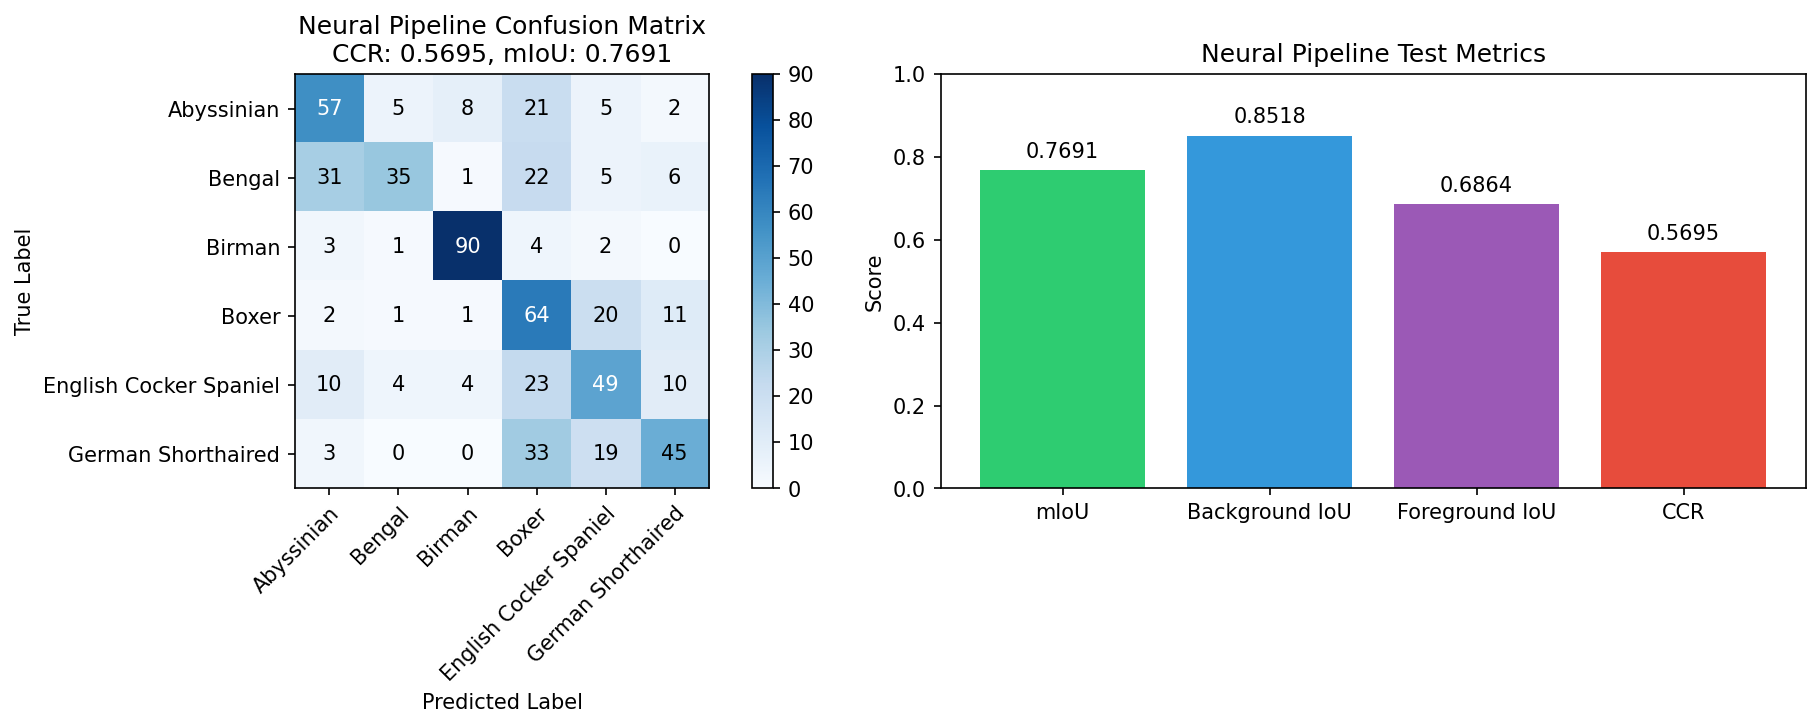
\includegraphics[width=0.75\textwidth]{assets/results_neural_test.png}
    \caption{Final neural pipeline metrics on test set: mIoU, CCR, and confusion matrix.}
    \label{fig:neural_results}
\end{figure}

The joint segmentation and classification training led to satisfactory mIoU and classification accuracy. The segmentation head helps the encoder focus on the animal.

\begin{figure}[H]
    \centering
    
\includegraphics[width=0.9\textwidth]{assets/segmentation_qualitative.png}
    \caption{Qualitative segmentation visualizations on test images: original image, ground-truth mask, CNN segmentation prediction.}
    \label{fig:segmentation_qualitative}
\end{figure}

\subsection{Traditional Pipeline (b)}
\phantomsection

Optimal K was selected based on validation (e.g., K=300, 400 or 500). Hyperparameters: M (e.g., 30000), MLP epochs=30, weight decay=1e-4, dropout=0.3.

Final metrics on test set for optimal K: \textbf{CCR} and \textbf{confusion matrix} (6$\times$6). Values are printed in the ``Traditional Pipeline Test Results'' and ``RESULTS SUMMARY'' cells of the notebook.

\begin{figure}[H]
    \centering
    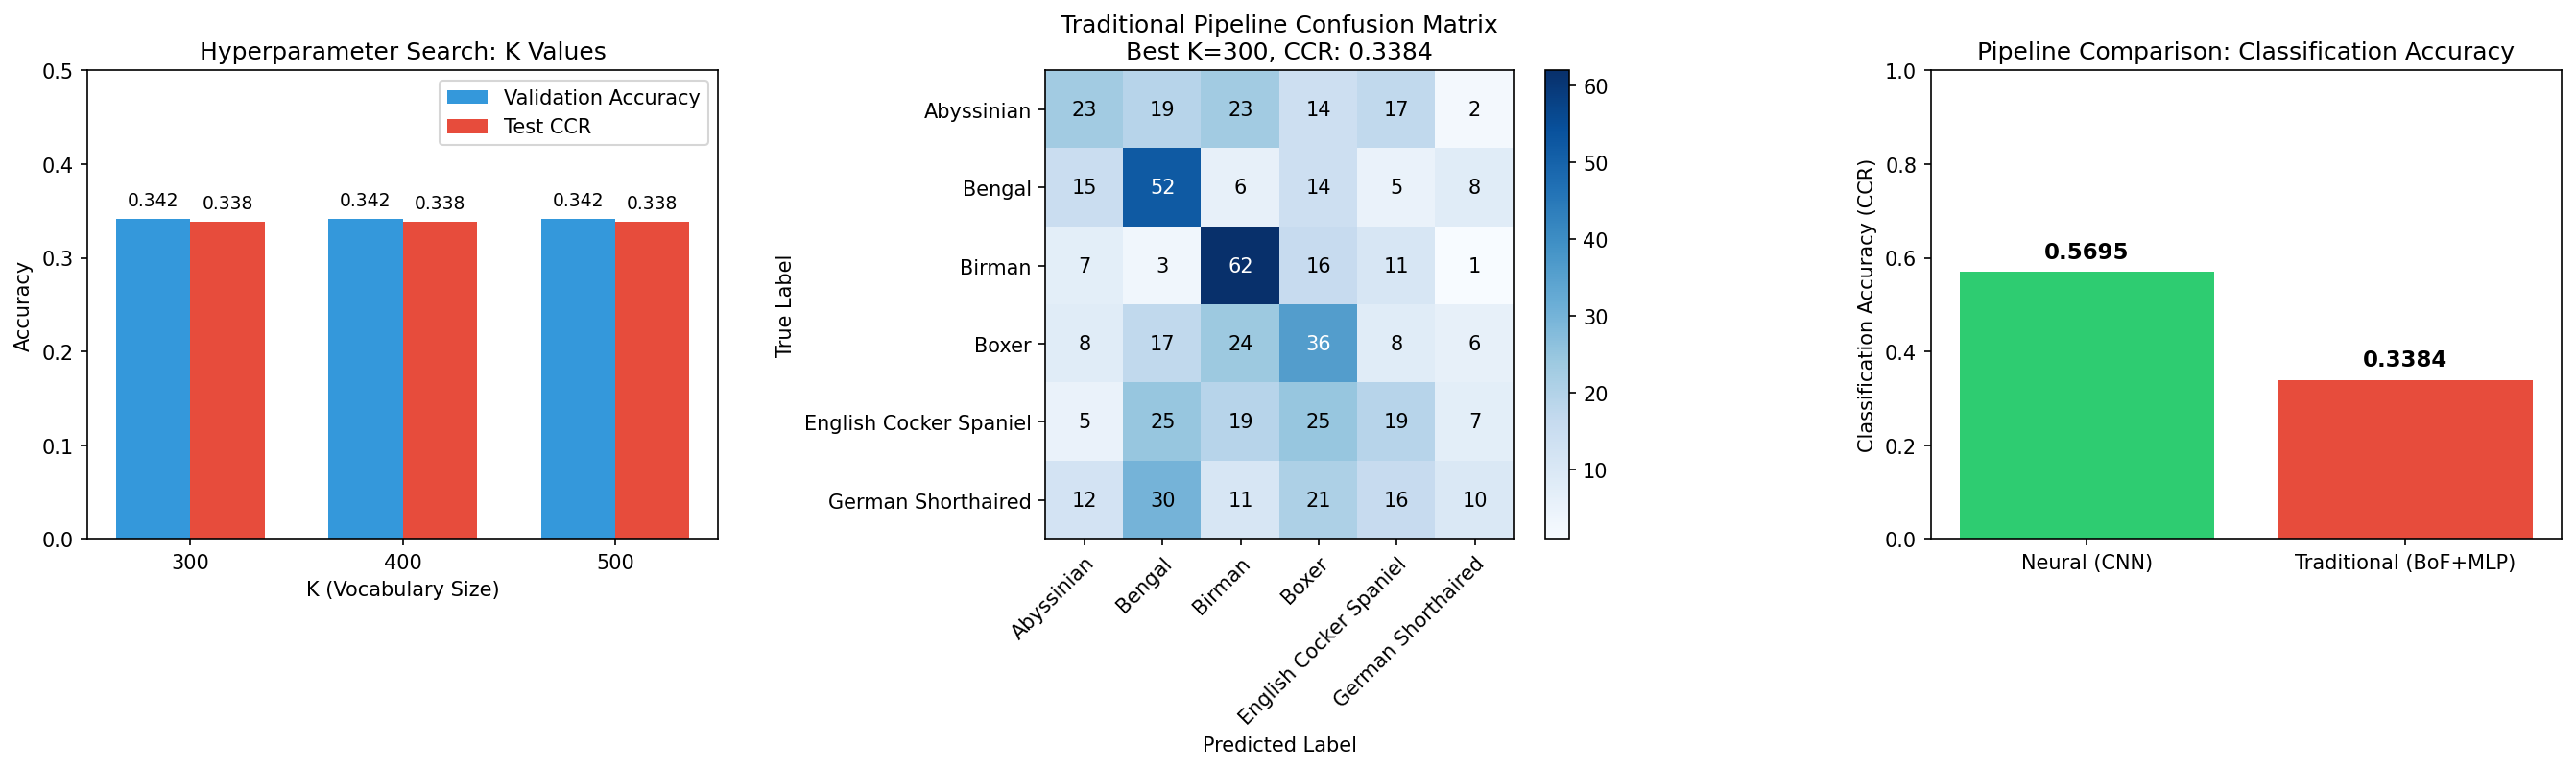
\includegraphics[width=0.75\textwidth]{assets/results_traditional_test.png}
    \caption{Final traditional pipeline metrics (optimal K) on test set: CCR and confusion matrix.}
    \label{fig:traditional_results}
\end{figure}

Comparatively, the neural model tends to achieve better classification accuracy thanks to learned features; BoF+MLP relies on SIFT and the fixed vocabulary.

\subsection{Background Replacement Verification (c)}
\phantomsection

On the test set with replaced background (low-frequency noise instead of original background), the CNN and MLP models were re-evaluated. The new \textbf{CCR} values are printed in the notebook (``Comparison: original test vs background-replaced test''). If models focus on the animal, CCR should remain close to original; a small drop indicates they also use information from the background.

\begin{figure}[H]
    \centering
    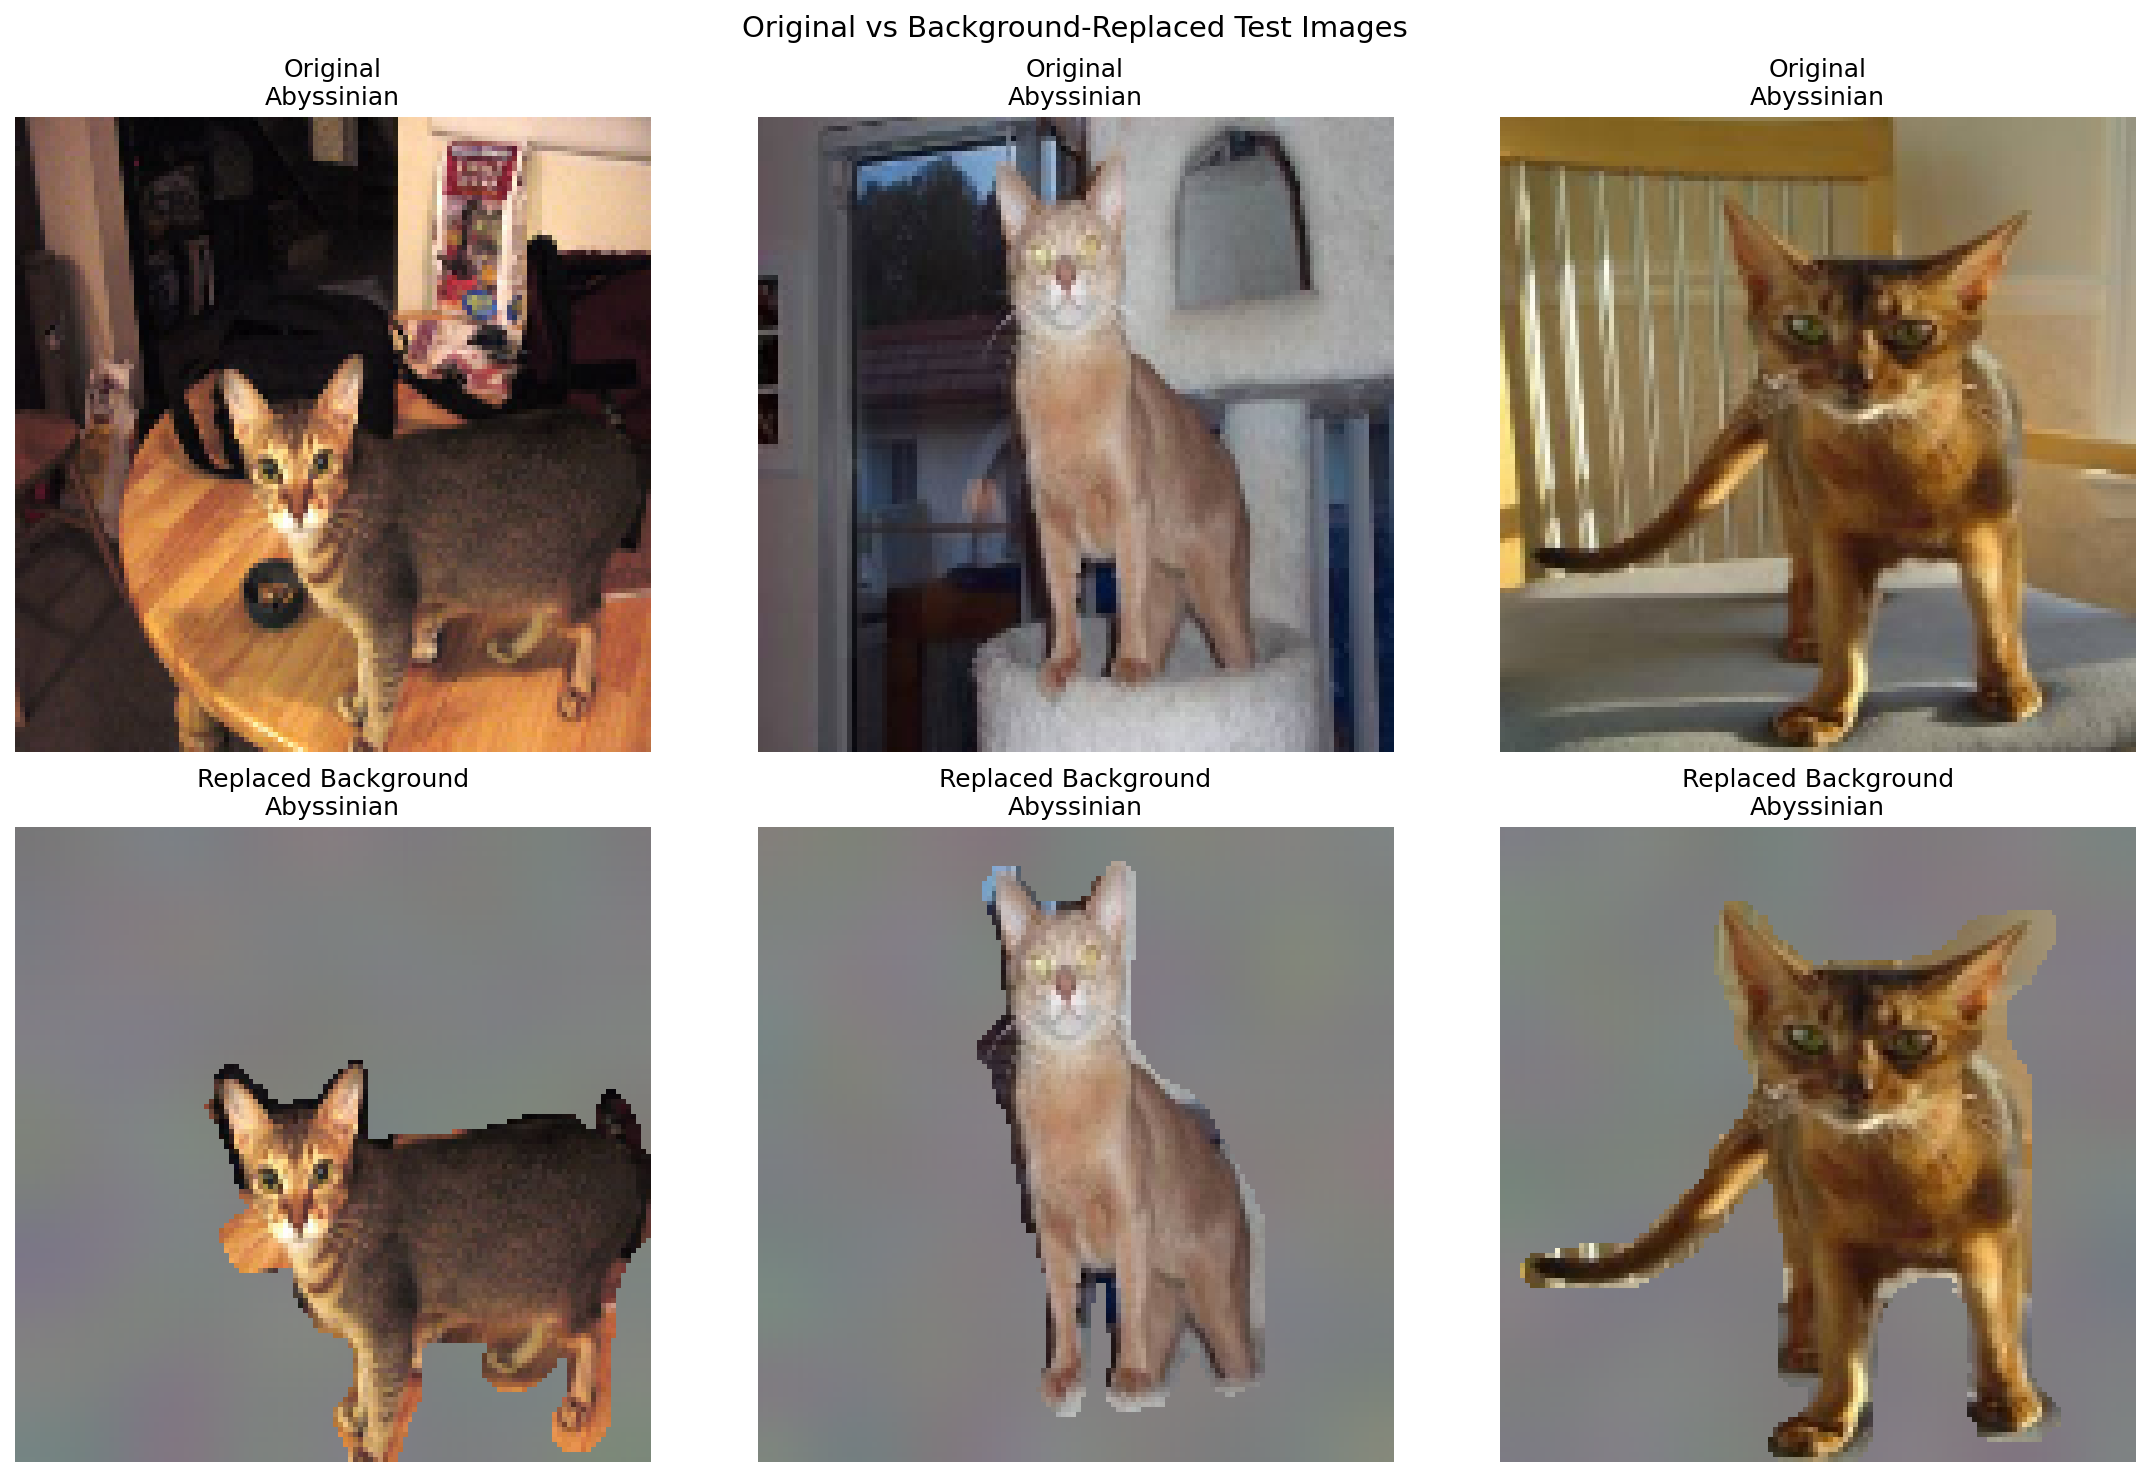
\includegraphics[width=0.7\textwidth]{assets/background_replaced_example.png}
    \caption{Example test image with replaced background (original vs.\ replaced background).}
    \label{fig:background_replaced}
\end{figure}

\begin{figure}[H]
    \centering
    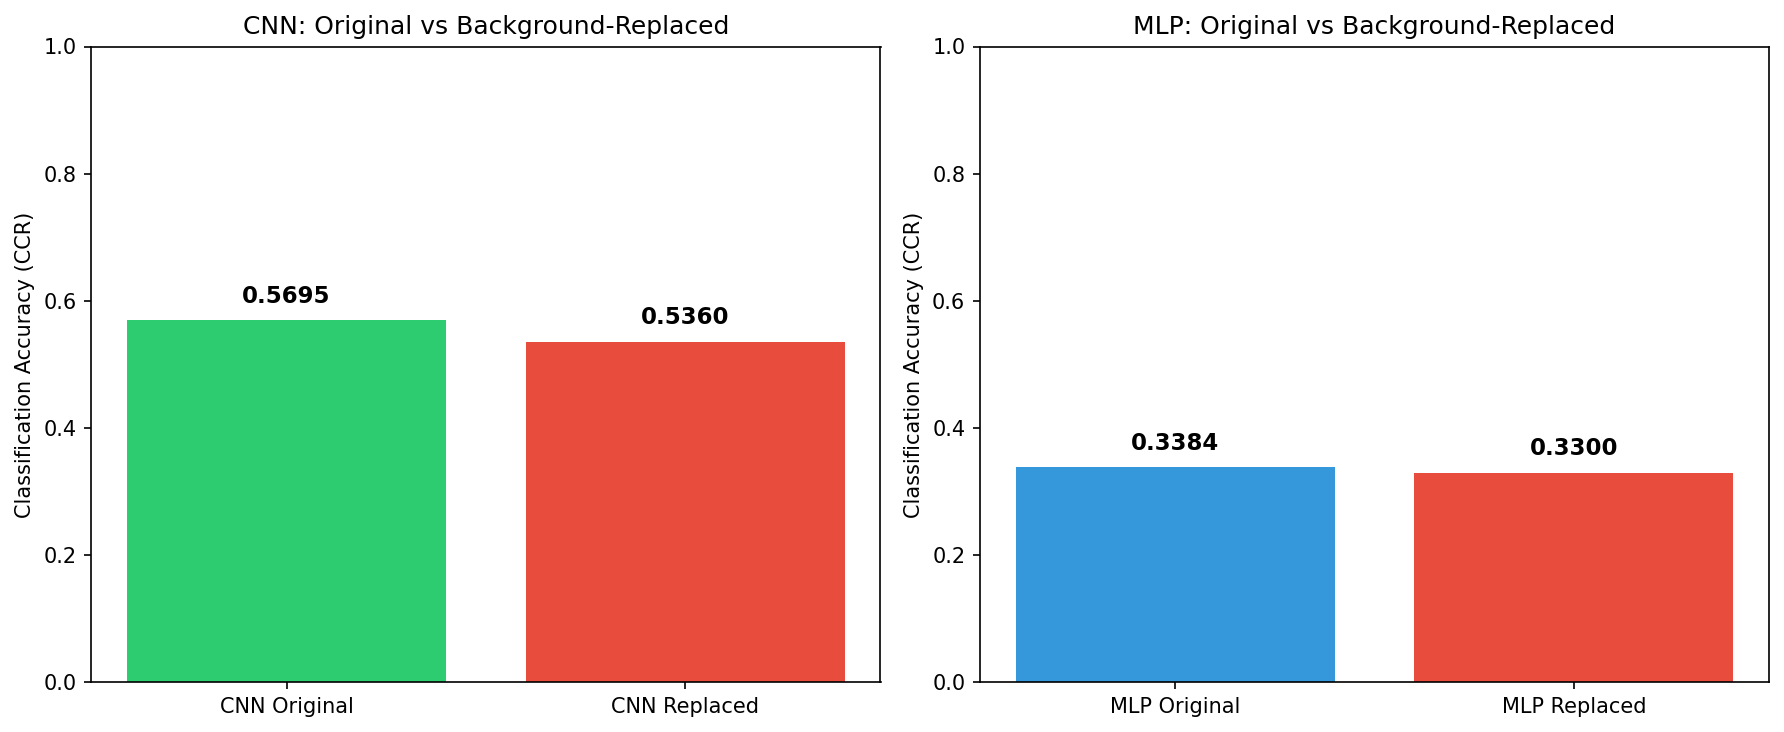
\includegraphics[width=0.8\textwidth]{assets/background_replaced_comparison.png}
    \caption{Comparison of classification accuracy (CCR) on original vs.\ background-replaced test sets for both CNN and MLP models.}
    \label{fig:background_replaced_comparison}
\end{figure}

\subsection{Summary and Discussion}
\phantomsection

What worked well: joint U-Net training with two heads; L1 normalization of BoF histograms; K selection with validation; manual metrics without external libraries. Challenges: CNN training time (reduced with 128$\times$128 and lightweight model); BoF sensitivity to vocabulary size and SIFT quality. Training was performed for 30 epochs for both models (CNN and MLP), according to the assignment.

\begin{figure}[H]
    \centering
    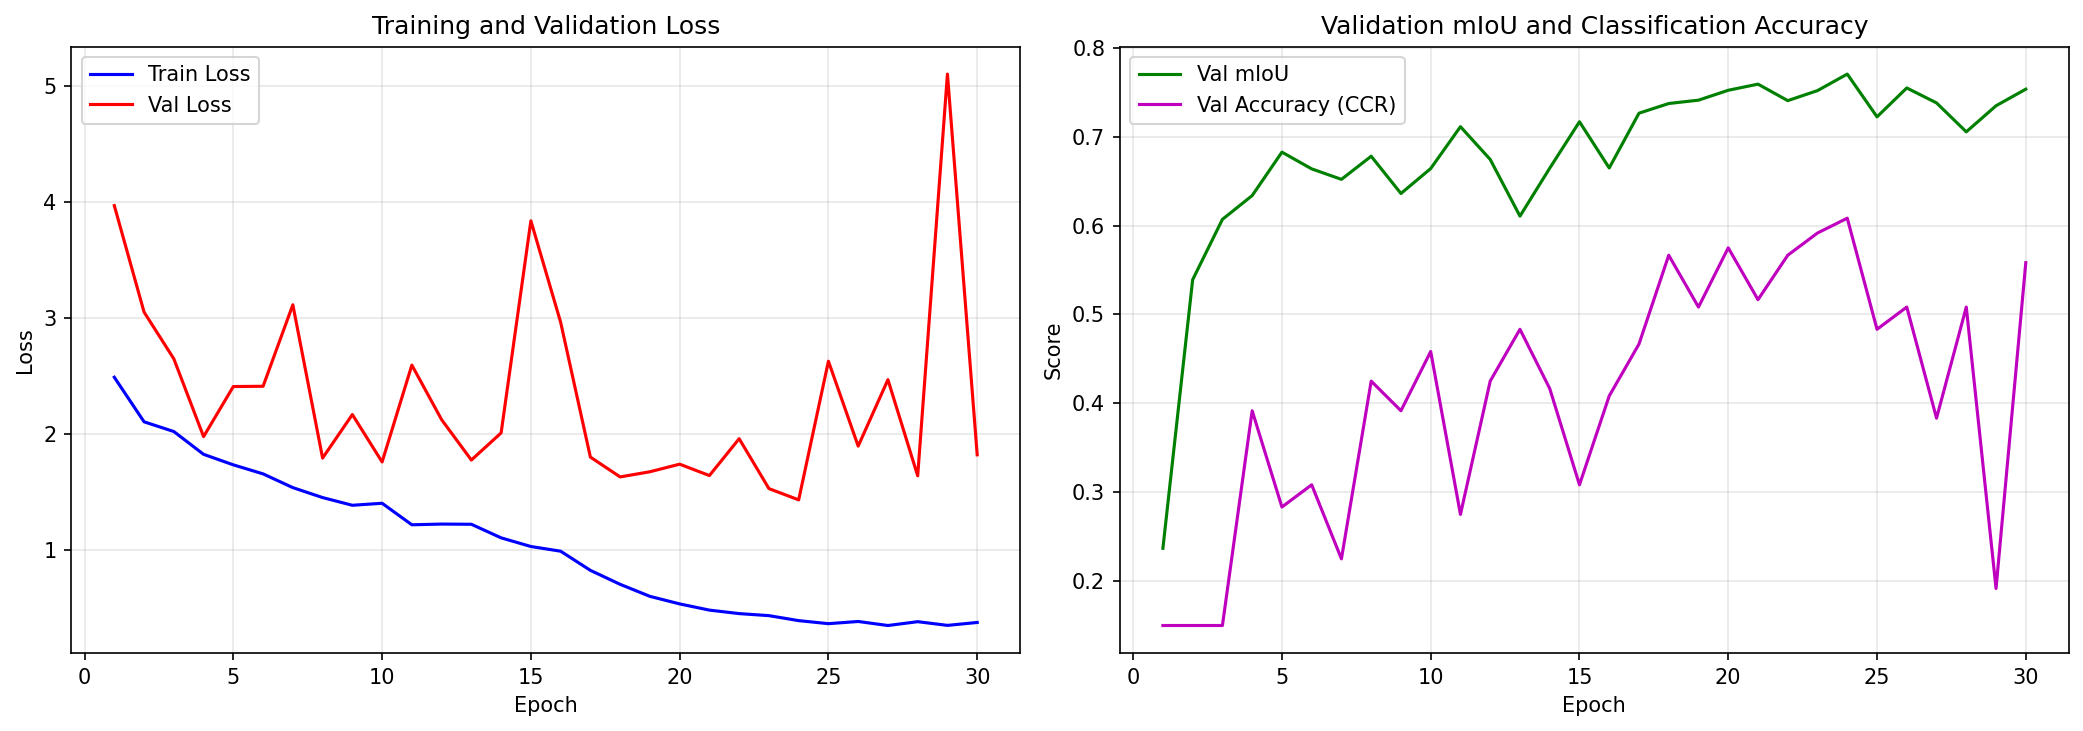
\includegraphics[width=0.8\textwidth]{assets/training_curves.png}
    \caption{Loss / accuracy plot over epochs for CNN or MLP.}
    \label{fig:training_curves}
\end{figure}

\section{Conclusion}
\label{sec:conclusion}
\phantomsection

The assignment covered two alternative classification approaches: neural (U-Net with dual head) and traditional (BoF + MLP). The main learnings were the importance of joint segmentation-classification training for better features, hyperparameter selection ($\lambda$, K) with validation, and verification that models focus on the animal through the background-replaced test.

\textbf{Limitations:} Small dataset size and only 6 classes; lightweight U-Net and low resolution (128) for speed; BoF depends on SIFT quality and vocabulary size.

\end{document}
